\section[image=bgphoto_cut]{Introduction}
\begin{frame}[plain]{}
    \sectionpage
\end{frame}

\begin{frame}{\tlap}
    \tlap is a high-level specification language for modeling concurrent and distributed digital systems:
    \begin{itemize}
        \item Algorithms
        \item Programs
        \item Complex computing systems
    \end{itemize}

    \tlap is based on set theory, first-order logic and the Temporal Logic of Actions (TLA); it uses ordinary, basic math.
\end{frame}

\begin{frame}{Leslie Lamport}
    \tlap is developed by Leslie Lamport
    \begin{itemize}
        \item Original author of \LaTeX, first release in 1984
        \item Fundamental contribution to the theory of distributed systems
        \begin{itemize}
            \item Logical Clocks
            \item Byzantine General's problem
            \item Chandy-Lamport distributed snapshot algorithm
            \item Paxos algorithm
            \item many, many other contributions
        \end{itemize}
        \item Turing Award in 2013 (and many other prizes)
    \end{itemize}
\end{frame}

\begin{frame}{\tlap tooling}
    \setbeamercovered{transparent}
    \begin{description}
        \item<1->[\tlap] specification language
        \item<1->[TLC] model checker and simulator of \tlap specs
        \item<-1>[PlusCal] algorithm language similar to a simple programming language, can be translated to \tlap
        \item<-1>[TLAPS] system for mechanically checking proofs written in \tlap
        \item<-1>[TLATeX] pretty-printer to typeset \tlap specifications in \LaTeX
        \item<1->[Toolbox] IDE for all the \tlap tools
    \end{description}
    \setbeamercovered{invisible}
    \pause
    \vspace{0.5cm}
    \begin{center}
        We will focus on \tlap and TLC and we will use the \tlap Toolbox
    \end{center}
\end{frame}

%TODO: history?

\begin{frame}{Motivations for simple, high-level language}
    Why should we use an high-level language which uses ordinary and simple math instead of some kind of programming language?
    \setbeamercovered{transparent}
    \begin{itemize}[<+->]
        \item It helps us abstract away from implementation details
        \item No special or new syntax, only simple math
        \item Specification of the system is written before the implementation, design errors are found as early as possible
        \item Specification is independent from the language used for implementation
    \end{itemize}
    \setbeamercovered{invisible}
\end{frame}

\begin{frame}{Industrial use of \tlap}
    Who uses \tlap?
    \setbeamercovered{transparent}
    \begin{itemize}
        \item<1> Intel
        \only<1>{
            \begin{itemize}
                \item Used since 2002
                \item Pre-RTL formal verification of cache-coherence protocol %TODO bib
            \end{itemize}
        }
        \item<2> Microsoft
        \only<2>{
            \begin{itemize}
                \item Used since 2004; usage increased in 2015 due to Azure
                \item Found subtle bugs in memory coherence protocol of Xbox 360, Cosmos DB, lock-free data structures
                \item Public specification of the consistency levels of Cosmos DB %TODO link to repo
            \end{itemize}
        }
        \item<3> OpenComRTOS
        \only<3>{
            \begin{itemize}
                \item New version of \emph{Virtuoso}, the OS of the European Space Agency's \emph{Rosetta} spacecraft
                \item \tlap specification helped to have a cleaner architecture, achieving 10x less code than Virtuoso %TODO bib
            \end{itemize}
        }
        \item<4> Amazon
        \only<4>{
            \begin{itemize}
                \item Used since 2011 for AWS (Amazon Web Services)
                \item As of 2014, used in 10 large complex systems %TODO bib
            \end{itemize}
        }
    \end{itemize}
    \setbeamercovered{invisible}
\end{frame}

\begin{frame}[plain]{Amazon}
    \begin{figure}
        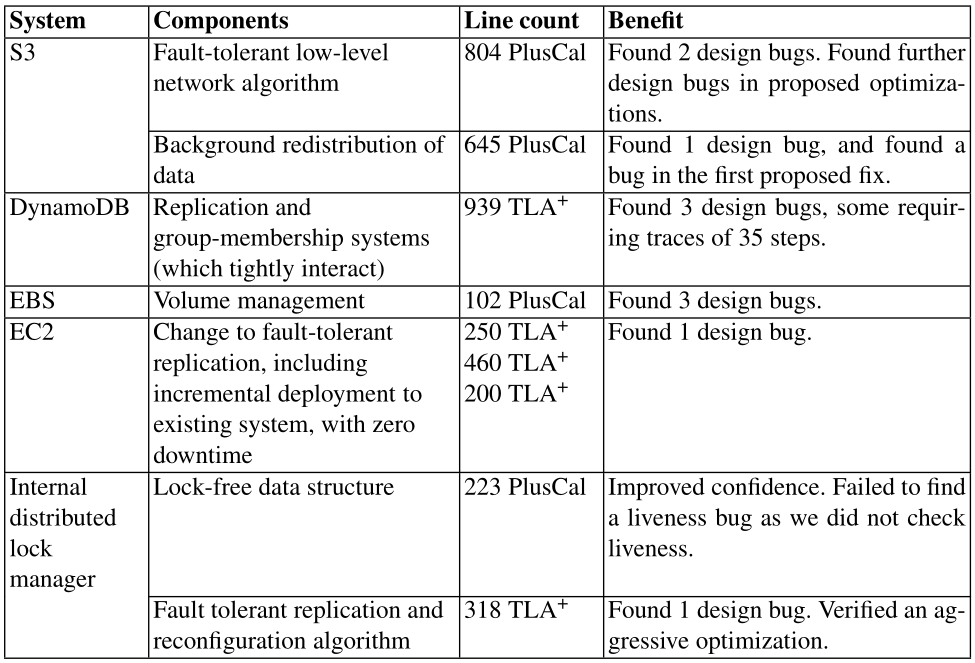
\includegraphics[width=0.9\textwidth]{images/amazon.png}
        \caption{\footnotesize Examples of \tlap usage at Amazon, from} %TODO bib
    \end{figure}
\end{frame}

\section[image=bgphoto_cut]{TLC}
\begin{frame}[plain]{}
    \sectionpage
\end{frame}

\begin{frame}{Specification}
    TLC can evaluate specifications that have the standard form
    \[
        Init \land \square \left[ Next \right]_{vars} \land Temporal
    \]

    where
    \begin{itemize}
        \item $Init$ is the initial predicate
        \item $Next$ is the next-state action
        \item $Temporal$ is a temporal formula (usually liveness conditions)
    \end{itemize}

\end{frame}

\begin{frame}{Temporal Formula}
    TLC can evaluate a temporal formula if it is a conjunction of the following classes of formulas:
    \begin{itemize}
        \item State Predicate
        \item Invariant ( $\square P$, where $P$ is state a predicate)
        \item Box-Action formula ($\square[A]_v$, where $A$ is an action)
        \item Simple Temporal Formula
    \end{itemize}
\end{frame}

\begin{frame}{Simple Temporal Formula}
    Given
    \begin{itemize}
        \item Simple boolean operators ($\land$, $\lor$, $\neg$, $\implies$, $\equiv$, $TRUE$, $FALSE$)
        \item Temporal state formula, that is a temporal formula obtained from state predicates by applying
        \begin{itemize}
            \item simple boolean operators
            \item temporal operators ($\square$, $\Diamond$, $\leadsto$)
        \end{itemize}
        \item Simple action formula\begin{align*}
            \WF_v \left( A \right) &&
            \SF_v \left( A \right) &&
            \square \Diamond \left< A \right>_v &&
            \Diamond \square \left[ A \right]_v &&
        \end{align*}
    \end{itemize}
    A simple temporal formula is defined as a formula constructed from temporal state formulas and simple action formulas by applying simple boolean operators
\end{frame}

\begin{frame}{TLC modes}
    TLC has two different modes
    \setbeamercovered{transparent}
    \begin{itemize}
        \item<1-> Model-checking mode
        \only<1> {
            \begin{enumerate}
                \item TLC computes all the initial states by evaluating $Init$
                \item TLC constructs the graph of all states of the system, using a BFS, by evaluating $Next$
                \item While expanding the graph, TLC checks that invariants and constraints are satisfied
                \item TLC checks that the temporal properties are satisfied
            \end{enumerate}
        }
        \item<2-> Simulation mode
        \only<2>{
            \begin{itemize}
                \item TLC repeatedly constructs and checks behaviors of the system that have a fixed maximum length
            \end{itemize}
        }
    \end{itemize}
    \setbeamercovered{invisible}
    \only<3>{
        Note that model-checking is possible only if the graph of the states is finite. If it is not finite, constraints to limit the number of states to be considered by TLC can be specified.
    }
\end{frame}